\chapter{Background}\label{chapter:background}
\glsresetall

\section{Overview}
This chapter provides the background necessary to understand the research presented in this thesis. We begin by introducing \glspl{cps}, which forms the primary application domain for our work. This includes discussions on safety-critical systems, timing analysis and \gls{wcet} analysis, and the distinction between real-time and synchronous execution models. We then present the fundamentals of \gls{ml}, particularly on \glspl{ann}, their training processes, evaluation metrics, and hyperparameter tuning techniques. 

We also cover explainability in \gls{ml}, introducing key techniques such as \gls{shap}, \gls{ale}, and Anchors essential for building explainable models. We then discuss formal modelling techniques, including \glspl{fsm}, \glspl{ta}, and Runtime Enforcement mechanisms that are important for verifying system safety and correctness. 

Following this technical foundation, we present the theoretical background on traditional model-based design and compositionality in \gls{cps}, examining how complex systems can be decomposed into manageable components. We then explore the current state of monolithic \gls{ml} approaches in \gls{cps}, focusing on their strengths in handling complex, nonlinear relationships and their limitations in verification, timing analysis, and explainability, and examine existing attempts to use compositional approaches to \gls{ml}-based \gls{cps} design.


\section{Cyber-physical Systems}

\glspl{cps} are digital systems that continuously interact with their physical environment. They consist of sensors, actuators and communicating devices that interact with each other and the physical world in a feedback loop \cite{alur_principles_2015}. CPSs consist of the physical process, the \emph{plant} and the embedded digital system, the \emph{controller}. A good example of a cyberphysical system will be an  \gls{av}, where the various sensors in the car are used by multiple connected controllers within the car to manoeuvre the car safely in its environment (the plant).

There are often safety-critical real-time systems, meaning they require \emph{firm} guarantees on their safety and timing behaviour \cite{tripakis_compositionality_2016}. For example, consider the task of lane changing in an  \gls{av}, which we use later as a case study. To make a successful lane change, the vehicle must sense the physical environment, such as the vehicles surrounding it, and determine when it is safe for the car to lane change based on learned behaviour. If the conditions are safe, inputs must be given to the digital car controls to manipulate the physical car components to execute a safe lane change. Thus, a functional and safe CPS needs control, computing, and communication to work together synergistically.



\subsection{Safety Critical System}
Embedded systems can be classified as safety-critical \cite{Doyen2018-st, 7104300} if their proper function is important to ensuring the safety of people around them.
A malfunction in these systems can lead to injury or even death. These systems require that they never produce an output that puts them in an unsafe state. Continuing the example of lane changing, which is a safety-critical system, it will mean that the car should never try to execute a lane change when there are cars next to it in the adjacent lanes.

It is crucial to verify the correctness of such a system to ensure safety. Verifying safety-critical systems often involves using high-level programming languages, as they allow for specifying the safety policies or specifications in an easy-to-understand and easy-to-code manner, which reduces the risk of errors in code logic. For example, easyRTE\footnote{https://github.com/PRETgroup/easy-rte} is one such tool that allows the safety specifications to be written in a programmer-friendly \emph{rte} language, which can then be invoked to ensure the runtime correctness of a system \cite{pearce_smart_2020}. 


\subsection{Timing Analysis and Worst-Case Execution Time}
The physical world is continuous, while the digital controller in a CPS is discrete in nature. This requires that the digital system respond to the changes in the physical environment in a timely fashion. This is known as the system's timing requirement. Real-time systems that require strict timing requirements or deadlines to ensure safe operation are termed as \emph{hard real-time} systems. Missing these timing deadlines can have grave consequences. Systems where a few timing requirements can be missed with little consequences are termed as \emph{soft real-time} \cite{wilhelm_worst-case_2008} systems.  

Generally, upper bounds on the execution time of such systems are needed to satisfy constraints for real-time systems with strict timing constraints. Timing analysis of real-time systems attempts to determine these bounds when a system is executed on a specific hardware \cite{wilhelm_worst-case_2008}. Assuming that a real-time system comprises a collection of tasks that achieve a standard functionality, the execution times of tasks vary with the input data or different environment behaviour \cite{wilhelm_worst-case_2008}. This variation results from the different paths different inputs may take within a task, depending on different conditions. 

Figure \ref{fig:wcet_time} shows an example variation of execution times depending on input data and environment factors. The blue curve represents the set of all execution times, whereas the orange curve represents the measured set of execution times. Thus, the longest execution time, in reality, is called the \gls{wcet}. It indicates a system's timing performance under the worst possible input and environment conditions \cite{wilhelm_worst-case_2008}.

\begin{figure}[htbp] 
 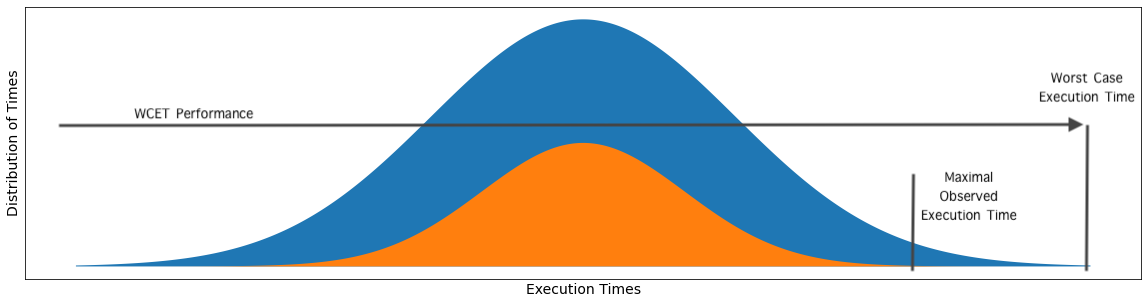
\includegraphics[width = \textwidth]{introduction/figures/WCET.png}
 \caption{Showing the distribution of example variation in execution times for a task as inputs and environment conditions change. The blue shaded region depicts the actual or real execution time variation, whereas the orange region represents the observed execution times.}
 \label{fig:wcet_time}
\end{figure}

As the execution time for a particular task depends on the path the control takes during a task and the time that statements and instructions spend on this path, the determination of WCET has to consider the potential control-flow paths and the execution times for this set of paths \cite{wilhelm_worst-case_2008}. There are two main approaches to timing analysis using WCET. First are Measurement-based methods that execute the task or task parts on the given hardware or a simulator for some set of inputs. Then, the maximal observed execution times are derived from the set of observed execution times. The worst maximal execution time is then used as the WCET. As expected, this method is limited by the type of inputs checked and can often provide an underestimation of the WCET \cite{wilhelm_worst-case_2008}.

On the other hand, Static methods do not depend on executing code on real hardware or a simulator. They instead take the task code itself, examine the set of possible control flow paths through the task, combine control flow with a (abstract) model of the hardware architecture, and obtain upper bounds (WCET) for this combination. Static methods emphasise safety by producing bounds on the execution time and guarantee that the execution time will not exceed these bounds. 

\subsection{Real-time and Synchronous Execution}
\label{sec:real_time_syn}

When multiple components in a CPS must interact, they must all advance in lock-step with wall-clock time. In purely software-based subsystems, this can be enforced via synchronisation signals. However, when real physical devices and computational models coexist, no single clock signal can span both domains. Instead, each element must honour \emph{real-time constraints} \cite{1012687}, meaning that its computation or physical action at every moment must complete in precisely the same duration as the corresponding simulated time.

Furthermore, a CPS must be \emph{reactive} to interact predictably with its environment. Conventional CPUs achieve reactivity either by \emph{polling}—continually checking inputs at regular intervals, which wastes cycles and can incur long delays—or by \emph{interrupts}, where a hardware signal forces an immediate change in program flow. While interrupts reduce idle CPU time, they complicate static timing analysis, often causing an explosion in the state space that must be examined. As a result, determining whether such systems meet hard real-time deadlines typically requires statistical simulations (e.g., Monte Carlo methods) that cannot exhaustively cover every path.

By contrast, synchronous execution adopts a discrete model of computation in which program behaviour is divided into atomic reactions separated by logical ticks \cite{berry_foundations_2000, boussinot_sl_1996}. At each tick, inputs are sampled instantaneously, internal computations occur atomically, and outputs are committed simultaneously at the tick's end. The implementation enforces a known \gls{wcet} per reaction so that logical time can be safely mapped to physical time. Unlike hardware interrupts—which may preempt execution arbitrarily and require context-save/restore—external events in the synchronous model are queued until the next tick boundary. At that point, the current reaction terminates cleanly and control transfers to the appropriate handler, without preserving any intermediate state. This provides a provable upper bound on response latency while keeping the state space small and deterministic.

Synchronous execution is ideal for embedded control where deterministic timing is non-negotiable, such as in safety-critical \gls{cps}. Its key advantages include:

\begin{itemize}
  \item \textbf{Deterministic Logical Time:} Rather than modelling continuous wall-clock time directly, the synchronous approach provides a logical clock and enforces that each reaction finishes within a known bound \cite{berry_foundations_2000,boussinot_sl_1996}. This yields a fully deterministic, formally analysable timing model. In contrast, continuous-time real-time systems must mirror physical time precisely—introducing hardware jitter, interrupt interference, and integration-solver uncertainties that are typically checked by empirical measurement rather than full formal proof \cite{buttazzo_hard_2011,kopetz_real-time_2011}.
  \item \textbf{Formal Deadline Guarantees:} As each synchronous reaction has a provable worst-case reaction-time bound (often mapped directly to its WCET on the target hardware), we can perform static schedulability analyses to guarantee deadlines \cite{liu_real-time_1973}. In continuous-time or \gls{rtos}-based systems—where tasks may be preempted by interrupts, use diverse clocks, or depend on \gls{os} scheduling—formal guarantees are far more complex and often require conservative benchmarks or runtime monitoring to ensure deadlines \cite{buttazzo_hard_2011}.
\end{itemize}


\section{Machine Learning}
As model-based design approaches to designing CPSs become unmanageable due to the complexity of the systems, we have seen a shift towards the use of data-driven models using Machine Learning (ML). Here, we discuss the basics of ML, particularly \glspl{ann}, and their training and evaluation processes. 

Broadly, ML is a field of \glspl{ai} that focuses on developing algorithms that allow mathematical models to learn from data and make decisions based on that data by learning patterns or representations in data \cite{murphy_machine_2012}. ML is used in a range of applications, such as natural language processing (\glspl{llm}),  speech recognition, and image recognition. In this work, we extensively use ML models (Artificial Neural Networks, in particular).



\subsection{Machine Learning Tasks}
The task of using mathematical algorithms to learn representations from data can be categorised into three main kinds: supervised learning, unsupervised learning, and reinforcement learning. Each of these types of learning has its own set of tasks and algorithms, and is used in different scenarios depending on the data and the problem at hand.

\textbf{Supervised Learning:} In Supervised learning, an ML model learns the input-output mapping from a set of labelled data. The model is trained on labelled data, where the input is the feature vector and the output is the label. The model then learns the relationship between the input and the output, and can predict the output for unseen data. 

The most commonly used supervised learning tasks are classification and regression. In classification tasks, the model learns to predict the class label of the input data, while in regression tasks, the model learns to predict a continuous value. The most common supervised learning algorithms are Decision Trees,  Ensemble Models like \glspl{rf},  \glspl{svm}, and \glspl{ann}. As we have labelled data, we will use ANNs for both classification and regression in this work, as ANNs have better representative power than other ML approaches.

\textbf{Unsupervised Learning:} Unsupervised learning is where the model learns the underlying structure of the data without any labels. The model is trained on an unlabelled dataset, where the input is the feature vector. The model then learns the relationship between the input data points and can group similar data points together. The most commonly used unsupervised learning tasks are clustering and dimensionality reduction. In clustering tasks, the model learns to group similar data points together, while in dimensionality reduction tasks, the model learns to reduce the number of features in the data.

\textbf{Reinforcement Learning:} Reinforcement learning teaches models when to take certain actions in an environment to maximise a reward signal. The reinforcement learning algorithm aims to learn a policy that maps the state of the environment to an action. The model is trained on a set of state-action-reward tuples, where the state is the current state of the environment, the action is the action taken by the model, and the reward is the reward signal received by the model. The model then learns the relationship between the state and the action, and can take actions to maximise the reward signal. The most common reinforcement learning tasks are game playing and robotics.


\subsection{Artificial Neural Networks}
Artificial Neural Networks (ANNs) are, as the name suggests, networks of artificial neurons that attempt to model the behaviour of biological neurons. ANNs use linear mathematical functions and nonlinear functions called activation functions to learn patterns or representations in data \cite{goodfellow_deep_2016}. ANNs are composed of layers of neurons, with each layer having a specific number of neurons. The first layer is called the input layer,  the layers in between are called hidden layers, and the last layer is called the output layer. The more layers an ANN has, the more \emph{deep} it becomes. Networks with multiple hidden layers are called \glspl{dnn}. DNNs are part of a subset of ML called \gls{dl}. Similarly, networks with one or fewer hidden layers are called a \emph{shallow} Neural Network. 

Most ANNs determine the untimed nonlinear relationships or mappings between a provided set of inputs and their corresponding outputs through a learning process called \emph{training}. This process manipulates the parameters/weights of an ANN to learn an accurate representation of the relationship between the inputs and the outputs. This ability allows them to perform tasks such as classification of input data, forecasting (regression), and language translation. The most common types of ANNs are \glspl{mlp}, \glspl{cnn}, and \glspl{rnn}. While ANNs can be used for supervised, unsupervised or reinforcement learning, we focus on their use in the supervised learning tasks of classification and regression. Also, we focus on \glspl{mlp} as they are the most common type of ANNs used in this work.


\subsubsection{Multilayer Perceptrons}
ANNs can be composed of artificial neurons of one or more types. \glspl{mlp} are the simplest kind of ANNs and are composed of perceptrons. Perceptrons are the simplest form of artificial neurons and are composed of a linear function followed by a nonlinear activation function. Mathematically, the output of a perceptron is given by Equation \ref{eq:perceptron}.

\begin{equation}
 \label{eq:perceptron}
 \textbf{Out} = f(\textbf{W}\cdot\textbf{In} + \textbf{B})
\end{equation}

where, $\textbf{Out}$ is the output of the perceptron; $\textbf{W}$ is the weights vector; $\textbf{In}$ is the input vector; $\textbf{B}$ is the bias vector; and $f$ is the nonlinear activation function. The weights and biases are learned during the training process.


The activation function $f$ is a nonlinear function that introduces nonlinearity into the output of the perceptron. This nonlinearity is crucial for the perceptron to learn complex nonlinear patterns in the data. Without the nonlinearity, the whole model will be reduced to a linear model, and the model will only learn linear relationships between the inputs and the outputs. The most common activation functions are Linear (Equation \ref{eq:linear}), Sigmoid (Equation \ref{eq:sigmoid}), \gls{tanh} (Equation \ref{eq:tanh}), ReLU (Rectified Linear Unit, (Equation \ref{eq:relu})) and Softmax (Equation \ref{eq:softmax}). The following are the mathematical expressions for these activation functions, in the same order.

\begin{equation}
 \label{eq:linear}
 f(x) = x
\end{equation}

\begin{equation}
 \label{eq:sigmoid}
 f(x) = \frac{1}{1 + e^{-x}}
\end{equation}

\begin{equation}
 \label{eq:tanh}
 f(x) = \frac{e^{x} - e^{-x}}{e^{x} + e^{-x}}
\end{equation}

\begin{equation}
 \label{eq:relu}
 f(x) = \max(0, x)
\end{equation}

\begin{equation}
 \label{eq:softmax}
 f(x_i) = \frac{e^{x_i}}{\sum_{j=1}^{n}{e^{x_j}}}
\end{equation}
 where $x_i$ is the $i$th element of the input vector, $x_j$ is the $j$th element of the input vector, and $n$ is the number of elements in the input vector.

While the choice of activation function rests on the problem at hand, the sigmoid is commonly used in the output layer of binary classification tasks. In contrast, softmax is used in the output layer of multi-class classification tasks. Linear, \gls{tanh}, and ReLU are primarily used in hidden layers of MLPs for regression and classification tasks. Linear activation functions are normally used in the output layer of regression tasks. 

MLPs are usually fully connected, meaning that all the neurons in a layer are connected to all the neurons in the next layer. Equation \ref{eq:ANN_out} expresses the mapping of inputs and outputs at layer $l$ of an MLP.

\begin{equation}
 \label{eq:ANN_out}
 \textbf{Out}^l = f^l(\textbf{W}^l.\textbf{Out}^{l-1} + \textbf{B}^l)
\end{equation}

where, $\textbf{Out}^l$ is the output vector produced by layer $l$; $\textbf{W}^l$ is the weights matrix for layer $l$; $\textbf{Out}^{l-1}$ is the input vector for layer $l$, which is the equal to the output from the previous layer $l-1$; $\textbf{B}^l$ is the bias vector; and $f^l$ is the nonlinear activation function for layer $l$. For the first layer $l=1$, the input to the network becomes the input to the layer. An MLP model is illustrated in Figure \ref{fig:ANN}.


\begin{figure}[htbp] 
 \centering
 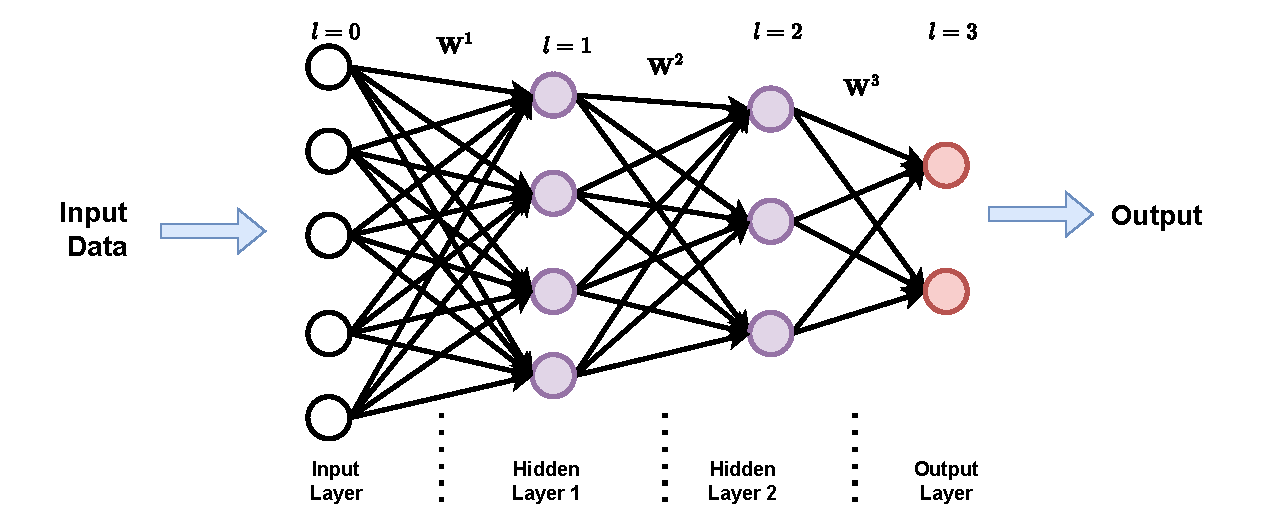
\includegraphics[width=\textwidth]{introduction/figures/ANN.pdf}
 \caption{A representative MLP model.}
 \label{fig:ANN}
\end{figure}


\subsubsection{Training}
ANNs \emph{learn} the representation of the input-output mapping through a process called training. During training, the ANN modifies the weights $\textbf{W}$ of the network such that a particular Cost function (also called Loss function) is optimised given a set of inputs or features and outputs. The loss function is usually a piecewise differentiable function of the true outputs and the outputs predicted by the network. It measures how much the predicted output deviates from the true output. The most common Loss function for classification is the Cross-entropy loss, defined as in Equation \ref{eq:crossentropy}. This is used in multi-class classification tasks.

\begin{equation}
 \label{eq:crossentropy}
 L_{CrossEntropy} = -\sum_{i=1}^{C}{y_i \cdot \log{\hat{y_i}}}
\end{equation}

where, $C$ is the number of classes in the data, $y_i$ is the expected class $i$ label/output, and $\hat{y_i}$ is the predicted output probability for a class $i$. For binary classification tasks, a special case of the Cross-entropy loss, the Binary Cross-entropy loss is used as shown in Equation \ref{eq:binarycrossentropy}.

\begin{equation}
 \label{eq:binarycrossentropy}
 L_{BinaryCrossEntropy} = -y \cdot \log{\hat{y}} - (1-y) \cdot \log{(1-\hat{y})}
\end{equation}


Moreover, in regression tasks, the Mean Squared Error (MSE) loss is used as shown in Equation \ref{eq:MSE}. Here, the goal is to minimise the difference or error between the expected and predicted output values, which are usually continuous values. 

\begin{equation}
 \label{eq:MSE}
 L_{MSE} = \frac{1}{n} \sum_{i=1}^{n}{(y_i - \hat{y_i})^2}
\end{equation}
where, $y_i$ is the expected output, and $\hat{y_i}$ is the predicted output. Here, $n$ is the number of samples in the dataset.

The optimisation of the Loss function is performed by an optimiser (such as \gls{adam} \cite{kingma2017adam}), which computes the ANN gradient in weight space with respect to the loss function. This gradient is then used to update the weights as shown in Equation \ref{eq:weightchange}.

\begin{equation}
 \label{eq:weightchange}
 \Delta \textbf{W} = \eta \frac{\delta \textbf{L}}{\delta \textbf{W}}
\end{equation}

where $\textbf{L}$ is the Loss function and $\eta$ is the learning rate that controls the magnitude of change in the weights.

This process of weight updation is called back-propagation. While the step of calculating the output across multiple layers using Equation \ref{eq:ANN_out} is called the forward pass, the weight updation step is called the backward pass. These two steps can be repeated iteratively until the desired Loss value or performance is obtained. If this process is not controlled correctly, the model may not converge to the desired output or overfit the data. Overfitting is a common problem in ANN models, where the model begins to learn the noise in the data rather than the actual input-output representation. This makes the model fail to generalise well to unseen but similar data. Normalisation of data and regularisation techniques can be used to prevent convergence issues and overfitting, respectively \cite{goodfellow_deep_2016}.


\textbf{Regularisation:} The problem of overfitting in ANNs is a common problem, and is usually solved using techniques such as dropout, early stopping, and regularisation during training. Dropout is a technique where a subset of neurons is randomly turned off during training, which helps in preventing the model from overfitting. Early stopping is a technique where the training is stopped when the model starts to overfit the data. Regularisation is a technique where a penalty term is added to the Loss function to prevent the model from learning complex patterns in the data. The most common regularisation techniques are L1 and L2 regularisation, which add the absolute and squared sum of the weights to the Loss function, respectively.

\textbf{Normalisation:} Often, the data used for training is normalised before it is sent to the ANN. This technique avoids the slower convergence of ANN models during training due to differences in scaling across features. While different scaling approaches are available, the most commonly used ones are Standard (or Z) scaling (see \ref{eq:standard_scaler}) and MinMax scaling (see \ref{eq:minmax_scaler}).

\begin{equation}
 \textbf{X} = \dfrac{\textbf{X} - {\boldsymbol{\mu}}}{{\boldsymbol{\sigma}}}
 \label{eq:standard_scaler}
\end{equation}


where $\textbf{X}$ is the matrix of input samples (excluding the labels), ${\boldsymbol{\mu}}$ is a vector containing the mean of the samples for each feature, and ${\boldsymbol{\sigma}}$ is the vector containing the standard deviation for the samples.

\begin{equation}
 \textbf{X} = \dfrac{\textbf{X} - \textbf{X}_{min}}{\textbf{X}_{max} - \textbf{X}_{min}}
 \label{eq:minmax_scaler}
\end{equation}

where $\textbf{X}_{min}$ and $\textbf{X}_{max}$ are the minimum and maximum values of the samples for each feature.

\textbf{Training Libraries:} Python libraries such as TensorFlow \cite{martin_abadi_tensorflow_2015} and PyTorch \cite{paszke_pytorch_2019} automate this process of training, and are often used by designers for ANN construction and training due to the simple API-based interface that these libraries provide. These tools provide means to define the ANN architecture, the Loss function, the optimiser, and the training parameters, and then train the model with a single function call. They also provide tools to control and monitor the training process, such as callbacks, which can be used to save the best model, reduce the learning rate, stop the training process early if the model starts to overfit the data, and regularise the model.



\subsubsection{Evaluation}
\label{sec:intro_evaluation}
Another part of ANN model development is the evaluation of the models developed. The evaluation is performed by measuring the model's performance on selected data using a set of metrics chosen based on the task at hand. These metrics try to ascertain the extent to which the model has learned the input-output representation in the data. In other words, the metrics measure how well the model output matches the expected (true) output.

For classification tasks, metrics such as accuracy, precision, recall, and F1 score are used. For regression tasks, metrics such as \gls{mse}, \gls{mae}, and R-squared are used. The following equations show the calculation of the metrics used in classification tasks.

\begin{equation}
 \label{eq:accuracy}
 Accuracy = \frac{TP + TN}{TP + TN + FP + FN}
\end{equation}

\begin{equation}
 \label{eq:precision}
 Precision = \frac{TP}{TP + FP}  
\end{equation}

\begin{equation}
 \label{eq:recall}
 Recall = \frac{TP}{TP + FN}
\end{equation}

\begin{equation}
 \label{eq:F1}
 F1 = 2 \cdot \frac{Precision\cdot Recall}{Precision + Recall}
\end{equation}

where, $TP$ is the number of True Positives, $TN$ is the number of True Negatives, $FP$ is the number of False Positives, and $FN$ is the number of False Negatives. Also, the following equations show the calculation of the metrics typically used in regression tasks.

\begin{equation}
 \label{eq:MSE_metric}
 MSE = \frac{1}{n} \sum_{i=1}^{n}{(y_i - \hat{y_i})^2}
\end{equation}

\begin{equation}
 \label{eq:MAE}
 MAE = \frac{1}{n} \sum_{i=1}^{n}{|y_i - \hat{y_i}|}
\end{equation}

\begin{equation}
 \label{eq:R2}
 R^2 = 1 - \frac{\sum_{i=1}^{n}{(y_i - \hat{y_i})^2}}{\sum_{i=1}^{n}{(y_i - \bar{y})^2}}
\end{equation}

where, $y_i$ is the expected output, $\hat{y_i}$ is the predicted output, and $\bar{y}$ is the mean of the expected output.


The choice of metric is crucial as it determines the performance of the model. For example, accuracy is not a good metric in a classification task when the classes are imbalanced. Take the case where we have 100 data points, of which 90 belong to a particular class. If a model predicts all the datapoints to belong to the majority class, the accuracy of the model will be 90\%. However, the model has not learned the input-output representation in the data. In such cases, metrics like the F1 score are preferred. Similarly, for regression tasks, the \gls{mse} is a good metric when the data does not have outliers or is normalised, while the \gls{mae} is a good metric when we want to obtain the error in the same range as the data.

Usually, the performance of a model is evaluated using a metric on a separate set of data called the test set, which is not used during the training process. This is done to ensure that the model generalises well to unseen data. However, this approach can lead to data-selection bias if the test set does not represent the data distribution. To avoid this, a technique called cross-validation is used. In cross-validation, the data is divided into $k$ folds, and the model is trained on $k-1$ folds and tested on the remaining fold. This process is repeated $k$ times, with each fold serving as the test set once. The model's performance is then averaged over the $k$ test folds to get a more accurate estimate of the model's performance. 5-fold \gls{cv} is one of the most commonly used techniques. We can also \emph{stratify} the data into folds to ensure that the folds have nearly the same proportion of the output variable/label. This is useful when the data is imbalanced \cite{goodfellow_deep_2016}.

\subsubsection{Hyperparameter Tuning}
Hyperparameters are parameters that control the model's learning process and can significantly impact the model's performance. Common hyperparameters include the learning rate, the number of layers in the model, the number of neurons in each layer, the activation function, the optimiser, the batch size, and the number of epochs. The process of finding the best hyperparameters for a model is called hyperparameter tuning. 

Tuning is usually performed using techniques such as grid search, random search, Bayesian optimisation or heuristic approaches like Evolutionary Algorithms. While Grid Search and Random Search are the most commonly used techniques, they are computationally expensive and time-consuming. They do not offer a guided search of the hyperparameter space and can be inefficient when the hyperparameter space is large. Hence, we focus on Bayesian Optimisation and Evolutionary Algorithms for hyperparameter tuning.

\textbf{Bayesian optimisation :} Bayesian optimisation is an advanced technique for hyperparameter tuning that is particularly effective when model evaluations are expensive or time-consuming. Instead of exhaustively searching the hyperparameter space, Bayesian optimisation builds a probabilistic surrogate model—commonly a Gaussian Process—to approximate the relationship between hyperparameters and the model's performance metric (such as accuracy or loss). This surrogate model is updated iteratively as new hyperparameter configurations are evaluated. This makes it especially useful for tuning complex models or when computational resources are limited \cite{frazier_tutorial_2018}.

\textbf{Evolutionary Algorithms:} Evolutionary Algorithms are a class of algorithms inspired by natural selection and evolution \cite{simon_evolutionary_2013}. These algorithms start with a random population of candidates and iteratively evolve the population using selection operators to choose the \emph{fittest} or most viable candidates. The process continues until a stopping criterion (usually based on a performance metric) is met. They offer a more guided and efficient search of the hyperparameter space compared to Grid Search and Random Search. Some of the most commonly used Evolutionary Algorithms are \glspl{pso} \cite{kennedy_particle_1995}, \glspl{de} \cite{storn_differential_1997}, and \glspl{es} \cite{emmerich_evolution_2018}.



\section{Explainability in Machine Learning}
\label{sec:intro_explainability}
While there is no mathematical definition for explainability\footnote{We use explainability and interpretability interchangeably in this work, as used in \cite{kamath_introduction_2021}.} regarding its use in Machine Learning, it is commonly accepted that it is the degree to which a human can understand and consistently predict the outputs of an ML model \cite{kamath_introduction_2021}. This is important for a number of reasons, including the need to understand the model's behaviour, to ensure that it is making decisions in a fair and unbiased way, and to build trust in the model. This is particularly important when using \emph{black-box} models (models for which it is too complex to understand their behaviour) used in high-stakes applications, such as healthcare.

We can broadly categorise explainability techniques into two categories: model-specific and model-agnostic. Model-specific techniques try to explain the decisions made by a specific model, while model-agnostic techniques can be applied to any model. Model-specific techniques include decision trees \cite{breiman_classification_2017}, which are easy to interpret but have limited expressive power, and \gls{ann}, which are difficult to interpret but can make more complex associations from multimodal data. 

Another way to categorise explainability techniques is by when they are applied: pre-hoc, in-hoc, and post-hoc \cite{molnar_interpretable_nodate}. Pre-hoc techniques are applied before the model is trained and include techniques such as feature selection and feature engineering \cite{guyon_introduction_2003}. In-hoc techniques are applied during the model training and include techniques such as attention mechanisms and saliency maps. 

Model-agnostic and post-hoc techniques, including Shapley Additive Explanations (SHAP) \cite{lundberg_unified_2017}, Accumulated Local Effects (ALE) \cite{apley_visualizing_2019}, and Anchors \cite{ribeiro_anchors_2018}, are particularly useful to interpret ANN outputs. In this section, we will discuss these techniques in more detail.


\subsection{Shapley Additive Explanations}
SHAP provides both local (explaining each prediction) and global (predictions over the entire dataset) explanations \cite{lundberg_unified_2017}. It computes the contribution of each feature to the prediction by linearly approximating the Shapley values. The computation of Shapley values for a feature $i$ is given by:

\begin{equation}
 \phi_i = \sum_{S \subseteq N \setminus \{i\}} \frac{|S|!(|N|-|S|-1)!}{|N|!} [f(S \cup \{i\}) - f(S)]
\end{equation}

where $N$ is the set of all features, $S$ is a subset of $N$, $f$ is the model, and $\phi_i$ is the SHAP value for feature $i$. 

SHAP simplifies the equation above and specifies an explanation as a linear model \cite{molnar_interpretable_nodate}. The SHAP value for a feature $i$ is given by:
\begin{equation}
 f(x) = \phi_0 + \sum_{i=1}^{M} \phi_i x_i
\end{equation}

where $f(x)$ is the model prediction, $\phi_0$ is the average prediction of the model - the prediction average over a background or reference dataset. Also, $\phi_i$ is the SHAP value for feature $i$, and $x_i$ is the feature value, and $M$ is the number of features.

As such, SHAP values are computed in relation to the average model prediction. Thus, a SHAP value of -0.4 for a feature in a sample, for instance,  means that the model prediction decreases by 0.4 from the average for a change in that feature. SHAP can be used to find the most important features of each participant. We get one SHAP value per data instance per feature and compute the mean of the absolute SHAP values for all instances in the dataset to obtain the overall SHAP value of a feature and the global feature importance for a model and a dataset. 


\subsection{Accumulated Local Effects}
ALE plots illustrate how specific features impact a model's predictions, with their values representing the main effect of a feature at a given point relative to the average prediction. Unlike some methods, ALE handles correlated features effectively \cite{apley_visualizing_2019}. We can determine using ALE plots how the most important features, as identified by SHAP, affect the model's predictions. These plots reveal how the effect of a feature on the prediction changes with different feature values, providing insight into whether an increase (or decrease) in the feature leads to a corresponding rise (or fall) in the model's prediction compared to the average.

The ALE values are computed in two steps. First, we compute the local effects. The local effects of Accumulated Local Effects are computed by dividing the feature into many intervals and computing the differences in the predictions. This procedure approximates the gradients and also works for models without gradients. First, we estimate the uncentered effect:
\begin{equation}
 \hat{\tilde{f}}_{j, ALE} = \sum_{k=1}^{k_j(x)} \frac{1}{n_j(k)} \sum_{i:x_j^{(i)} \in N_j(k)} [f(z_{k,j}, x_{\backslash j}^{(i)}) - f(z_{k-1,j}, x_{\backslash j}^{(i)})] 
\end{equation}

where $f$ is the model, $x$ is the data instance, $j$ is the feature, $k$ is the interval, $N_j(k)$ is the set of instances in the $k$th interval, $z_{k,j}$ is the $k$th interval value, and $n_j(k)$ is the number of instances in the $k$th interval.

Second, the uncentered effect is centred so that the mean effect is at zero \cite{molnar_interpretable_nodate}. The centred effect is given by:

\begin{equation}
 \hat{f}_{j, ALE} = \hat{\tilde{f}}_{j, ALE} - \frac{1}{n} \sum_{i=1}^{n} \hat{\tilde{f}}_{j, ALE} (x_j^{(i)})
\end{equation}

where, $\hat{f}_{j, ALE}$ denotes the centred Accumulated Local Effect for feature $j$ at a specific value. The term $\hat{\tilde{f}}_{j, ALE}$ represents the uncentered Accumulated Local Effect, which reflects the sum of local changes in the model's prediction attributable to feature $j$. The second term, $\frac{1}{n} \sum_{i=1}^{n} \hat{\tilde{f}}_{j, ALE} (x_j^{(i)})$, computes the mean uncentered effect across all $n$ data instances, where $x_j^{(i)}$ is the value of feature $j$ for the $i$-th instance. Subtracting this mean centres the ALE values so that their average effect over the dataset is zero, making interpretation relative to the average model prediction easier.

The value of the centred ALE can be understood as the main effect of the feature at a specific value compared to the average prediction of the data. For example, an ALE estimate of -4 at $x_j$ = 6 means that when the $j^{th}$ feature has a value of 6, then the prediction is lower by four compared to the average prediction.


\subsection{Anchors}
Anchors provide explanations for a prediction made by any black-box classification model by identifying an IF-THEN decision rule that sufficiently \emph{anchors} the prediction \cite{ribeiro_anchors_2018}. A rule is considered to anchor the prediction if changes in other features do not change the outcome. Additionally, anchors incorporate the concept of coverage, indicating the range of other, potentially unseen, instances to which the explanation applies.

We can define an anchor A formally  as follows:
\begin{equation}
 \mathbb{E}_{D_x(z|A)}[1_{f(x) = f(z)}] \geq \tau, A(x) = 1
\end{equation}

where $x$ is the instance being explained, $D_x(z|A)$ is the distribution of perturbations to $x$ that satisfy the anchor $A$, $f$ is the classification model, $\tau$ is the precision threshold, and $A(x)$ is a set of predicates, i.e., the resulting rule or anchor, such that $A(x)=1$ when all feature predicates defined by $A$ correspond to $x$'s feature values.

The above definition is impossible to solve, so a probabilistic definition is used in practice.
\begin{equation}
 P(prec(A) \geq \tau) \geq 1 - \delta, \text{ with } prec(A) = \mathbb{E}_{D_x(z|A)}[1_{f(x) = f(z)}]
\end{equation}

Here, $prec(A)$ denotes the precision of the anchor $A$, which is the expected proportion of perturbed instances that retain the same prediction as the original instance $x$. The threshold $\tau$ is the minimum required precision for an anchor to be considered valid. The parameter $\delta$ represents the statistical confidence level, ensuring that the probability the precision is at least $\tau$ is no less than $1-\delta$.

Moreover, coverage is formally defined as an anchor's probability of applying to its neighbours, i.e., its perturbation space. Coverage is given by:

\begin{equation}
 cov(A) = \mathbb{E}_{D_{(z)}}[A(z)]
\end{equation}

In the above equation, $cov(A)$ represents the coverage of the anchor $A$. The term $\mathbb{E}$ indicates the expected value, and $D_{(z)}$ refers to the distribution over perturbed instances $z$. The function $A(z)$ is an indicator function that equals $1$ if the anchor $A$ applies to the instance $z$, and $0$ otherwise. Thus, the coverage measures the proportion of instances in the local neighbourhood of the explained instance for which the anchor conditions hold true.


Hence, to get the anchors with coverage, we optimise the following:

\begin{equation}
 \max_{A s.t. P(prec(A) \geq \tau)\geq 1 - \delta} cov(A)
\end{equation}


We can use Anchors to show how predictions for classification models can be explained in a rule-based manner. This can be useful for understanding the model's behaviour and building trust in the model.


\section{Formal Modelling Techniques}
Formal modelling techniques are needed to describe the properties of a CPS. These techniques help describe the behaviour of the system and its environment in a mathematically precise manner. These mathematical models can then be verified using verification software with proven correctness guarantees. In this section, we will discuss three formal models: Finite State Machines, Timed Automata, and Valued Discrete Timed Automata. We will also briefly cover a formal verification approach called Runtime Enforcement.

\subsection{Finite State Machines}
A Finite State machine (FSM) is a mathematical model extensively used in formal modelling and verification, and is also known as a finite-state automaton. At any point in time, the model can be in one of a finite number of states. The \gls{fsm} execution starts at its \emph{initial} state and progresses to other states based on the inputs to the model - this process is called a \emph{transition}. When the model can only transition to one other state based on a specific set of inputs, the model is said to be a deterministic \gls{fsm}. On the other hand, if the model can transition to more than one state given the same set of inputs, the model is said to be a non-deterministic \gls{fsm}. The discrete states in an \gls{fsm} allow for the control flow of a system or property to be broken down into logical sections, making it easier to understand and verify the system's behaviour.


\begin{figure}[htbp] 
 \centering
 \begin{tikzpicture}[->,shorten >=1pt,auto,node distance=1.5cm,
 semithick, initial where=below]
 \tikzstyle{every node}=[font=\small]
 \tikzstyle{good state}=[circle,thick,draw=blue!75,fill=blue!20,minimum size=5mm,accepting]
 \tikzstyle{bad state}=[circle,thick,draw=red!75,fill=red!20,minimum size=3mm]
 \tikzstyle{dead state}=[rectangle,thick,draw=red!75,fill=red!20,minimum size=5mm]

 \node[initial, good state] (l0) {$Locked$};
 \node[good state]  at (6,0) (l1) {$Unlocked$};

 \path (l0) edge node {$Coin$}( l1)
 (l0) edge [loop above] node { $Push$ } (l0) 
 (l1) edge [bend left] node { $Push$ } (l0)
 (l1) edge  [loop above] node {$Coin$} (l1);
 \end{tikzpicture}
 \caption{An \gls{fsm} for a coin-operated turnstile.}
 \label{fig:fsm}
\end{figure}

For example, consider the case of a coin-operated turnstile. Here, the control starts at the \emph{Locked} location. If a coin is inserted, the control moves to the \emph{Unlocked} location. If the turnstile is pushed, the control moves back to the \emph{Locked} location. This can be modelled as an \gls{fsm} with two states: \emph{Locked} and \emph{Unlocked}. The \gls{fsm} can be represented as in Figure \ref{fig:fsm}. The system remains in an unlocked state as long as the coins keep getting inserted. Also, the control can only move to \emph{Unlocked} state if a coin is inserted; pushing the turnstile without inserting a coin will not change the state of the system.





\subsection{Timed Automata}
There are times when a system or property behaviour may depend on the time taken to perform certain actions. In such cases, a \gls{ta} can be used to model the system or property. A timed-automaton is constructed by adding a finite set of real-valued clocks to a \gls{fsm}. Multiple real-valued clocks can be defined, and they can be initialised from zero and reset to zero to measure the time taken for an action to occur. The clocks can also be used to define time constraints on the transitions between states. 


\begin{figure}[htbp] \label{fig:ta}
 \centering
 \begin{tikzpicture}[->,shorten >=1pt,auto,node distance=1.5cm,
semithick, initial where=below]
 \tikzstyle{every node}=[font=\small]
 \tikzstyle{good state}=[circle,thick,draw=blue!75,fill=blue!20,minimum size=5mm,accepting]
 \tikzstyle{bad state}=[circle,thick,draw=red!75,fill=red!20,minimum size=3mm]
 \tikzstyle{dead state}=[rectangle,thick,draw=red!75,fill=red!20,minimum size=5mm]

 \node[initial, good state] (l0) {$Locked$};
 \node[good state]  at (6,0) (l1) {$Unlocked$};

 \path (l0) edge node {$Coin; x: = 0$}( l1)
 (l0) edge [loop above] node { $Push$ } (l0)
 (l1) edge [bend left] node { $Push \lor x > 5$ } (l0)
 (l1) edge  [loop above] node {$Coin \lor x \leq 5$} (l1);
 \end{tikzpicture}
 \caption{A TA for a coin-operated turnstile.}
 \label{fig:ta}
\end{figure}

An example of a simple TA is shown in Figure \ref{fig:ta}, which is an extension of the \gls{fsm} in Figure \ref{fig:fsm}. Here, the system remains in the \emph{Unlocked} state for a maximum of 5 time units after a coin is inserted. If the turnstile is pushed within this time, the system moves back to the \emph{Locked} state. However, if the turnstile is not pushed within 5 time units, the system moves to the \emph{Locked} state anyway. The TA can be used to model the time taken for the turnstile to be pushed after a coin is inserted.

\subsection{Valued Discrete Timed Automata}

A \gls{vdta} is an automaton characterised by a finite set of locations, a finite collection of discrete clocks to track temporal evolution, and external variables—which correspond to input and output channels—that represent the system's data flows \cite{pearce_smart_2020}. In addition to these external variables, VDTAs include internal variables to carry out computations, whereas external variables simply capture data exchanged between the monitored system and its environment.

VDTAs operate on an implicit logical tick, much like synchronous programming languages \cite{benveniste_synchronous_2003}. Every transition is defined with respect to this tick: at the tick's start, all inputs are sampled, and at its end, all outputs are produced. This tick thus embodies one atomic reaction of the reactive system. As the majority of this work uses synchronous semantics, \glspl{vdta} will be used to model system specifications. Complete semantics of the \gls{vdta} can be found in \cite{pearce_smart_2020}.



\subsection{Runtime Enforcement}
It is not always possible to model the entire system behaviour using formal methods due to the complexity of the system. \gls{re} can be used in such cases to ensure the system behaves as expected. \gls{re} monitors the system's behaviour at runtime and ensures that the system satisfies certain policies. If the system violates the policies, \gls{re} takes corrective action to bring the system back to a safe state.

Runtime enforcement can be implemented using a monitor that observes the system's behaviour and checks if the system is adhering to the specified policies. If the system violates the policies, the monitor can take corrective actions to bring the system back to a safe state. The monitor is constructed as a formal model (such as \glspl{fsm}, \glspl{ta}, and \glspl{vdta}). The monitor can be used to check the system's behaviour against the specified policies and take corrective actions if the system violates the policies. The monitor can be implemented as a separate module that runs alongside the system and checks the system's behaviour periodically. If the monitor detects a violation, it can send a signal to the system to take corrective actions.


\begin{figure}[htbp] 
 \centering
 \begin{tikzpicture}[->,shorten >=1pt,auto,node distance=1.5cm,
 semithick, initial where=below]  
 \tikzstyle{every node}=[font=\small]
 \tikzstyle{good state}=[circle,thick,draw=blue!75,fill=blue!20,minimum size=20mm,accepting]
 \tikzstyle{bad state}=[circle,thick,draw=red!75,fill=red!20,minimum size=10mm]
 \tikzstyle{dead state}=[rectangle,thick,draw=red!75,fill=red!20,minimum size=10mm]

 \node[initial,good state] (l0) {$l_0$};
 \node[dead state] at (6,0) (l1) {$l_1$};

 \path (l0) edge node {$\neg P \land N $}( l1)
 edge [loop above] node { $(P \land N) \lor (P \land \neg N)$ } (l0)
 edge [loop left] node { $\neg P \land \neg N$ } (l0)
 (l1) edge  [loop above] node {$\Sigma$} (l1);

 \end{tikzpicture}
 \caption{Runtime enforcement monitor (\gls{vdta}) for lane change system in an  \gls{av}.}
 \label{fig:re}
\end{figure}

Figure \ref{fig:re} shows an example of a runtime enforcement monitor for the lane change system in an  \gls{av}. The monitor checks that the car should not make a lane change when the safety property $P$ is not satisfied and the lane change model $N$ suggests a lane change. In all other cases, the system stays in the safe state $l_0$. If the monitor detects an imminent violation (i.e., transition to $l_1$), it updates the output of the lane change module ($N \rightarrow \neg N$) so that no lane change can occur. 


Having established the technical foundations of \glspl{cps}, \gls{ml}, explainability, and formal modelling, we now turn to the principles of compositionality that underpin the design of complex systems. These compositional principles, originally developed in the context of model-based design, provide the theoretical basis for the compositional \gls{ml} framework developed in this thesis. We also examine how data-driven models have been used in \glspl{cps} and the challenges that arise from their monolithic design.


\section{Cyber-Physical Systems and Compositionality}

Designing \glspl{cps} by iterative trial and error—building prototypes, testing them, discovering faults, and revising—remains the most common approach \cite{tripakis_compositionality_2016}. Although this method is straightforward, it is both expensive and potentially unsafe: flaws detected late in development are costly to remedy, and defects that only surface after deployment can jeopardise human safety. In many industries, post-release fixes are now routine—from over-the-air software patches in consumer electronics to vehicle recalls in the automotive sector and device corrections in medical equipment.

\subsection{Model-based Design of CPS}

To overcome the drawbacks of the trial-and-error approach, \gls{mbd} emerged as a more disciplined alternative \cite{Nicolescu2018-vj}. In this approach, engineers develop abstract models, ranging from simple spreadsheets to fully executable simulations, that emulate key aspects of the target system. These models offer several benefits. They eliminate the risks associated with experimenting on real hardware, reduce costs by requiring fewer resources than building full prototypes, and enable rapid, scalable testing through simulations that can be run in parallel for extensive coverage within tight schedules. Furthermore, formal verification techniques applied to models can exhaustively explore system behaviours, uncovering corner-case errors before implementation. The process of correcting a model is typically simpler and less expensive than modifying physical prototypes.


However, models are abstractions and inevitably introduce simplifications. Ensuring that these approximations do not invalidate analysis results demands careful management of model fidelity—a central scientific challenge in system design.

At its core, \gls{mbd} addresses three fundamental questions \cite{tripakis_compositionality_2016}:
\begin{enumerate}
  \item \textbf{Modelling :} How can we precisely and efficiently capture the essential characteristics of the system under design? Creating accurate models is inherently difficult, especially across diverse engineering domains—mechanical, chemical, biological, and beyond. Each field has developed its own specialised modelling languages, modelling algorithms, and tools, but within the context of MBD.
  \item \textbf{Analysis:} Does the model satisfy the intended requirements—functionally, temporally, and economically? After constructing a model, the next step is to verify that it meets its specifications, covering correctness, performance, reliability, and cost metrics. As systems become complex, closed-form analytic methods often become infeasible, and \emph{computer-aided techniques} such as model checking rise to prominence.

 In model checking, one frames a system model \(S\) and a formal policy \(\varphi\) (expressed, for example, in temporal logic) and then automatically determines whether the system satisfies the policy \(S \models \varphi\). If not, the tool produces a counterexample illustrating the violation. Temporal logics distinguish between Safety (e.g., "always \(p\)" means that \(p\) never fails) and Liveness policies (e.g., "eventually \(p\)" asserts that \(p\) will occur at some point).
  
 The principal obstacle in formal verification is the \emph{state-explosion problem}: even modest systems can yield astronomically large state spaces, exacerbated further by continuous or hybrid dynamics. Although undecidability is a problem for rich models, ongoing research continuously extends the reach of practical verification tools through abstraction, compositional techniques, and heuristic optimisations.
  
  \item \textbf{Implementation:} By what processes can we transform the verified model into a deployable system, while preserving its certified properties? Ultimately, a verified model must be translated into an executable system. \emph{Automated code generation} frameworks already exist in industry, but they must meet a critical requirement: \emph{semantic preservation}. That is, the generated code should faithfully implement the behaviours that the model was proven to exhibit. Perfect preservation—down to real-number arithmetic—is typically impossible on finite-precision hardware. Nonetheless, one can often identify and guarantee the \emph{essential properties} needed for correct operation, while relaxing or approximating secondary aspects. 
\end{enumerate}




\subsection{Compositionality in Model-Based Design}
\label{sec:lit_compositionality}

Contemporary definitions of a "system" that merge state and dynamics into one monolithic entity become unwieldy for large-scale systems, such as modern automobiles, aircraft, or complex biological organisms. Capturing every possible state and transition in a single model (i.e., a \emph{monolithic model}) is impractical. Instead, we decompose a complex system into smaller subsystems, each of which may itself be further subdivided \cite{De_Roever2006-fx}. 

There are multiple paradigms for how subsystems communicate and synchronise:
\begin{enumerate}
  \item \textbf{Synchronous composition}, where all subsystems advance in lock-step, and every transition occurs simultaneously across components.
  \item \textbf{Asynchronous (interleaving) composition}, where at most one component transitions at any given moment, leaving the others unchanged.
\end{enumerate}

\begin{figure}[htbp] 
  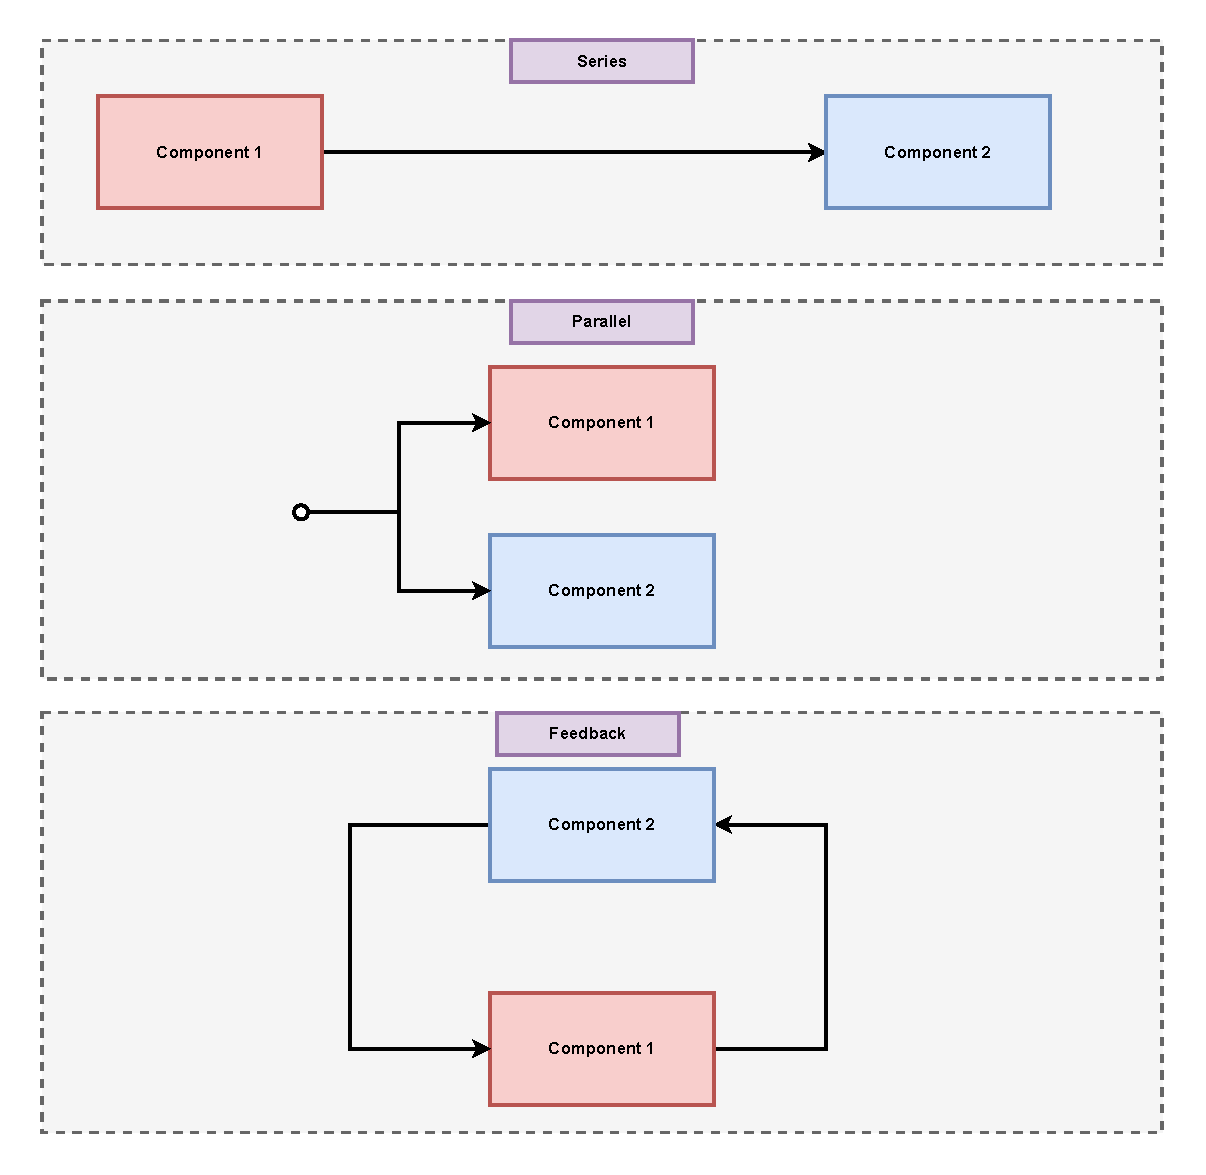
\includegraphics[width=\textwidth]{lit_review/fig/tripakis_compositionality.pdf}
  \caption{Composition of subsystems.}
  \label{fig:compositionality_tripakis}
\end{figure}

Beyond timing considerations, subsystems may be connected in series, in parallel, or via feedback loops, as shown in Figure \ref{fig:compositionality_tripakis}\footnote{We consider systems with a static structure. Dynamic systems are useful in several fields, including biology and economics, but are not considered in this work.}. Depending on the modelling framework, these "connections" can represent zero-delay wires, message queues (e.g., FIFO buffers in dataflow models), or shared-memory constructs typical of multithreaded software \cite{tripakis_compositionality_2016}.

Generally, we see compositionality as serving two main purposes. First, it helps us tame complexity by building sophisticated systems out of simpler components. Second, it addresses heterogeneity by enabling the integration of systems of different kinds \cite{1173203}. Compositionality in system design thus divides into two main themes:
\begin{enumerate}
  \item \textbf{Scalability of analysis:}  Can we infer global system properties by examining individual components? Techniques such as assume-guarantee reasoning and refinement allow us to conclude that the composed system inherits the desired properties if each component satisfies its contract (or refines a specification).
  \item \textbf{Modularity and reuse:}  Can we replace one subsystem with an equivalent one without re-verifying the entire assembly? Well-defined interfaces abstract away internal details, exposing only what is necessary for correct interaction, thereby enabling safe replacement, extension, and reuse of components.
\end{enumerate}

Together, these compositional principles underpin a systematic approach to designing, verifying, and evolving complex engineered systems. The following section summarises how data-driven \gls{ml} models are used in \glspl{cps} and the main barriers to their verification and deployment; Chapter \ref{chapter:lit_review} then reviews the related literature in detail.


\section{Data-driven Models in CPS}
\label{sec:lit_ann_cps}

\subsection{ML-based Models in CPS}

As the complexity of engineered systems continues to grow, traditional model-driven design approaches that rely on detailed physical process modelling are becoming increasingly impractical and difficult to scale. This is particularly true for \glspl{cps}, where the intricate interplay between computational and physical components leads to highly complex and often poorly understood dynamics. In such contexts, constructing accurate, first-principles models of the underlying processes can be prohibitively time-consuming, require significant domain expertise, and may fail to capture all relevant behaviours or uncertainties in real-world environments.

In response to the challenges, data-driven techniques for system design have emerged as a compelling alternative \cite{alzubaidi_rain-aware_nodate, xing_ensemble_2020, wang_bayesian_2021}. Among these, ML models like \glspl{ann} have gained significant prominence due to their remarkable ability to approximate complex, nonlinear input-output relationships directly from data, without the need for explicit knowledge of the system's internal dynamics \cite{goodfellow_deep_2016}. ML models are particularly well-suited for tasks where the mapping from inputs to outputs is difficult to express analytically, or the system is subject to variability and noise that are hard to model using traditional methods. 

For example, in autonomous vehicles, an ML-based classifier can be trained to recognise potential lane-changing opportunities by learning from large datasets of driving scenarios. Rather than relying on a hand-crafted set of rules or a detailed physical model of vehicle-environment interactions, the ANN can directly infer the relevant patterns and decision boundaries from sensor data, such as camera images, lidar point clouds, or radar signals. This data-driven approach enables the system to adapt to a wide range of conditions and edge cases that might be difficult to anticipate or encode explicitly, thereby enhancing the flexibility and robustness of CPS design.

Among all models, ANN models have found the most applications in \glspl{cps} due to their ability to approximate complex nonlinear relationships and their ability to be trained on large datasets. The body of work using ANNs far exceeds the body of work using other models, and we will primarily focus on ANN-based literature. We will now look at the errors, explainability, and verification barriers of ML-based (particularly ANN-based) \glspl{cps}.


\subsection{Errors, Explainability, and Verification Barriers}

ML-based systems are often prone to a variety of errors \cite{huang_safety_2017}. These errors can arise from several sources, including overfitting to training data, poor generalisation to unseen scenarios, and sensitivity to small input perturbations (adversarial examples) \cite{goodfellow_explaining_2015}. Additionally, data-driven models may suffer from distributional shifts, where the operational environment differs from the training data, leading to unexpected or unsafe behaviours \cite{moreno_unifying_2012}. 

Consider the paper in \cite{goodfellow_explaining_2015}, where the authors show how adding properly chosen noise can cause a model to misclassify an image. If an  \gls{av} is using a similar ANN to make a decision, it could potentially cause a crash. Errors can also result from incomplete or biased training datasets \cite{torralba_unbiased_2011}, mislabelled data, or insufficient model capacity to capture the true system dynamics. Furthermore, implementation issues such as quantisation errors, numerical instability \cite{sze_efficient_2017}, and hardware-induced faults can further degrade the reliability of ANN-based systems, especially in safety- and time-critical applications.

The deployment of ML models like \glspl{ann} in real-time, safety-critical, and time-critical application domains imposes stringent requirements for formal guarantees regarding both their functional correctness \cite{clarke_jr_model_2018} and their timing behaviour \cite{mitra_time-critical_2018}. In these domains, it is not sufficient for an ML model to perform well on average; it must be possible to provide rigorous assurances that the network will always behave as intended, within specified time constraints, under all possible operating conditions. Various formal verification techniques have been developed and proposed to address these needs for ANNs \cite{woodcock_formal_2009}. However, the formal verification of ANNs is known to be an NP-Complete problem \cite{katz_reluplex_2017}, making it computationally intractable for medium to large-scale networks.

A significant barrier to the widespread adoption of formal verification methods for ANNs is the prevalent design paradigm in which these networks are constructed and implemented as large, monolithic black-box \cite{yang_compositional_2020} models. In such monolithic architectures, the entire functionality is encapsulated within a single, often very large, network, with little or no internal modularity or structure that can be exploited for analysis. These monolithic ANN designs are typically characterised by their substantial size, high computational and memory requirements, and slow execution times \cite{yang_compositional_2020}. They are also resource-intensive, demanding significant hardware resources for training and inference, and are rarely amenable to parallelisation or incremental development and verification \cite{tripakis_compositionality_2016}.

As a result, the formal verification of monolithic ANNs often necessitates the use of substantial approximations \cite{ehlers_formal_2017} or the development of complex abstraction techniques \cite{gehr_ai2_2018} to make the problem tractable. These approximations and abstractions, while sometimes effective, can introduce conservatism or incompleteness, potentially undermining the strength of the guarantees that can be provided. 

Furthermore, the sheer size and complexity of monolithic ANN designs impose practical limitations on their implementation, particularly when targeting affordable custom hardware platforms such as \glspl{fpga} for timing analysis - due to their deterministic timing behaviour. In practice, this means that only relatively small networks—often comprising just a few tens of neurons—can be feasibly implemented on such hardware, as demonstrated in studies such as \cite{saric_fpga-based_2020} and \cite{nguyen_efficient_2018}. This hardware constraint further restricts the applicability of monolithic ANN designs in resource-constrained, safety- and time-critical systems, highlighting the need for alternative, more modular approaches.


\section{Summary}

This chapter introduced the background needed for the remainder of the thesis. We defined \glspl{cps} as safety-critical, real-time systems that require timely and correct interaction between physical plants and digital controllers, and explained why \gls{wcet} analysis and synchronous execution are relevant when timing guarantees matter. We then summarised core \gls{ml} concepts, with emphasis on feedforward \glspl{ann}, their training and evaluation, and post-hoc explainability techniques (\gls{shap}, \gls{ale}, and Anchors). Formal modelling tools---including \glspl{fsm}, timed automata, and runtime enforcement---were presented as mechanisms for specifying and monitoring system behaviour.

On the design side, we contrasted model-based compositionality in \gls{cps} with the growing use of data-driven \glspl{ann} in control applications. We discussed typical ML failure modes, the difficulty of verifying monolithic networks, and practical hardware limits on implementing them for timing analysis on resource-constrained platforms.
